\subsection{Objective of the project}
The object of the project is to study the color chaos model that was paper published by Prof. Ping Chen in the paper \cite{pchen}. The approach of this paper is to understand the mathematical concepts of color chaos, time frequency analysis - Wigner distribution and Gabor transformation.  In the paper \cite{pchen}, the S\&P 500 composite monthly index price was taken for the analysis, and in this project the color chaos model is studied for both the S\&P 500 and NASDAQ indices.

\subsection{Organization of Project}
This report has been organized into five chapters. Chapter 1 outlines the entire project giving an introduction to time series forecasting using stochastic models. Chapter 2 introduces Fourier transformation, discrete Fourier transformation, Gabor transformation and joint time-frequency analysis. Chapter 3 provides an overview of Wigner distribution. Chapter 4 introduces the Time-frequency distribution series (TFDS) and chapter 5 introduces color chaos and contains the conclusion of the study.

\subsection{Data Source:}

The color chaos model is evaluated for two indices in this study and the sources of the data for the indices are given below in table ~\ref{table:datasource}. 

\begin{table}[h!]
\centering
\begin{tabular}{||c c c c c||} 
 \hline
 Symbol & Description & Source & Frequency & Duration \\ [0.5ex] 
 \hline\hline
 FSPCOM & S\&P 500 Price Composite index & Citibase & Monthly & 1942-1992 \\ 
 NASDAQ & NASDAQ Composite index & Yahoo Finance & Monthly & 1970-2016 \\ 
 \hline
\end{tabular}
\caption{Meta data on FSPCOM(S\&P 500) \& NASDAQ}
\label{table:datasource}
\end{table}


\begin{figure}[!ht]
\centering
\includegraphics[scale=.15]{Images/RawData}
\caption{Data used in the study. a) Actual SP500 and log(SP500) b) Actual NASDAQ and log(NASDAQ). The matlab program drawDataGraph.m used to generate the graph is given in Appendix A}
\label{fig:rawdata}
\end{figure}

\subsection{Time series forecasting using stochastic models}
In general, models for time series data can have many forms and represent different stochastic processes. The most widely used linear time series models are Auto Regressive (AR) and Moving Average (MA) models. Combining these two, the Autoregressive and Moving Average (ARMA) and Autoregressive Integrated Moving Average (ARIMA) are also used. The Autoregressive Fractionally Integrated Moving Average (ARFIMA) model generalized ARMA and ARIMA models. For seasonal time series forecasting, a variation of ARIMA, the Seasonal Autoregressive Integrated Moving Average (SARIMA) model is used. 

Linear models have drawn much attention due to their relative simplicity in understanding and implementation. Many practical time series show non-linear patterns. Non-linear models are appropriate for predicting the volatility changes in economic and financial time series. Considering these facts, various non linear models have been proposed over the years. A few widely used non-linear models are Autoregressive Conditional Heteroskedasticity (ARCH) model, its variations like Generalized ARCH (GARCH), Exponential GARCH (EGARCH), the Threshold Autoregressive (TAR), the Non-linear AutoRegressive (NAR), the Non-linear Moving Average (NMA) model and others. 

The Autoregressive Moving Average (ARMA) models:
An ARMA(p,q) model is a combination of AR($p$) and MA$(q)$ models and is suitable for univariate time series modeling. In an AR(p) model the future value of a variable is assumed to be a linear combination of p past observations and a random error together with a constant term. 

Mathematically the AR(p) model can be expressed as:
\begin{equation}
y_t = c+\sum_{i=1}^{p} \varphi_{i} y_{t-i}+\epsilon_{t}
\end{equation}

Here $y_t$ and $\epsilon_t$ are the actual value and random error respectively at time period $t$, $\varphi_{i} (i=1,2,3,....,p)$ are model parameters and $c$ is a constant. The integer constant $p$ is known as the order of the model. Sometimes the constant term is omitted for simplicity. A AR$(p)$ model regresses against past values of the series; an MA$(q)$ model uses past errors as the explanatory variables. The MA$(q)$ model is given by

\begin{equation}
y_t = \mu+\sum_{j=1}^{q} \theta_{j} \epsilon_{t-j} + \epsilon_{t}
\end{equation}

Here $\mu$ is the mean of the series, $\theta_j (j=1,2,3,...q)$ are the model parameters and $q$ is the order of the model. The random shocks are assumed to be a white noise process, i.e. a sequence of independent and identically distributed (i.i.d) random variables with zero mean and a constant variance $\sigma^{2}$. Generally, the random shocks are assumed to follow a normal distribution. Conceptually a moving average model is a linear regression of the current observation of the time series against the random shocks of one or more prior observations. Fitting an MA model to a time series is more complicated than fitting an AR model because in the former one the random error terms are not fore-seeable.  Autoregressive (AR) and moving average (MA) models can be effectively combined together to form a general and useful class of time series models, known as ARMA models. Mathematically an ARMA$(p,q)$ model is represented as:

\begin{equation}
y_t = c+\epsilon_{t}+\sum_{i=1}^{p} \varphi_{i} y_{t-i} +\sum_{j=1}^{q} \theta_{j} \epsilon_{t-j}
\end{equation}

Here the model orders $p,q$ refer to $p$ autoregressive and $q$ moving average terms. 

\subsection{Difference Stationary }
Loosely speaking a stationary process is one whose statistical properties do not change over time. More formally, a strictly stationary stochastic process is one where given $t_1,....t_l$ the joint statistical distribution of $X_{t_1},...,X_{t_l}$ is the same as the joint statistical distribution of $X_{t_l+\tau}$ for all $l$ and $\tau$. It means that all moments of all degrees (expectations, variances, third order and higher) of the process anywhere are the same. It also means that the joint distribution of $(X_t,X_s)$ is the same as $(X_{t+\tau},X_{s+\tau})$.

A stochastic process is said to be stationary if its mean and variance are constant over time. i.e. time invariant. A stationary process will not drift too far away from its mean value because of the finite variance. 

Difference Stationary: Sometimes even de-trending is not sufficient to make a time series stationary, in such case, it may be necessary to transform it into a series of period-to-period and/or season-to-season differences to make the series stationary. Such a series is said to be difference-stationary.


If the trend in a time series is a deterministic function of time, such as $t$ or $t^2$, we call it a deterministic (predictable) trend. If it is not predictable, we have a stochastic trend. 

Consider the following model. 

\begin{equation}
Y_t = \alpha +\beta_{1}t +\beta_{2}Y_{t-1}+u_t 
\end{equation}

where $u_t$ is white noise.

\textbf{Pure Random Walk:} $\alpha = 0$, $\beta_1$=0, and $\beta_2$=1. This is non stationary as we get $Y_t = Y_{t-1} + u_t$. The mean is constant over the time, but the variance is increasing linearly with time. If we find the difference, we get $\Delta Y_t$= $u_t$. Note that differenced series is stationary (DS) because \textit{$E(\Delta Y_t) = E(u_t) =0$ } and \textit { $Var(\Delta Y_t) = Var(u_t) = \sigma^2$}. Both are time invariant. Hence, a random walk without a drift is difference-stationary(DS).


\textbf{Random Walk with a drift:} $\alpha \neq 0, \beta_1=0$, and $\beta_2$=1. This is non stationary as we get $Y_t = Y_{t-1} + u_t + \alpha$. The mean and variance are both increasing linearly with time. If we find the difference, we get $\Delta Y_t$= $\alpha + u_t$. Note that differenced series is stationary (DS) because \textit{$ E(\Delta Y_t)= E(\alpha + u_t) =\alpha$} and \textit {$Var(\Delta Y_t) = Var(u_t) = \sigma^2$}. Both are time invariant. Hence, a random walk with a drift is also difference-stationary(DS). $Y_t$ is trending upward or downward depending on the sign of the drift $(\alpha)$.

\begin{figure}[!ht]
\centering
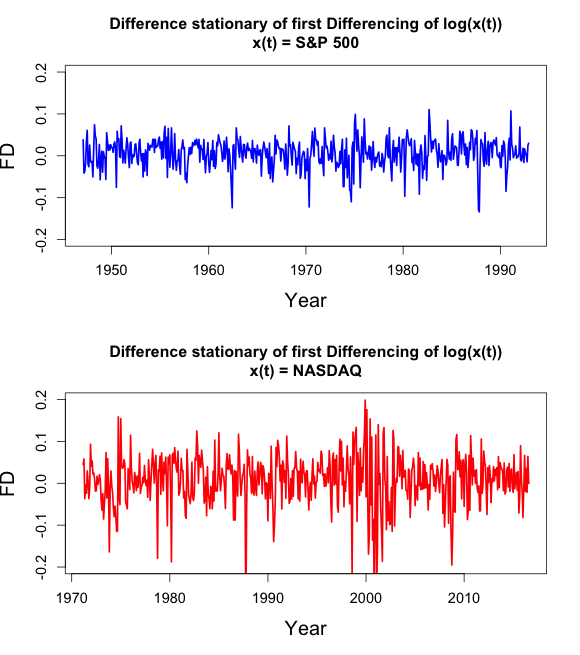
\includegraphics[scale=.65]{Images/DS}
\caption{Difference stationary of natural log a) SP500 b) NASDAQ.The difference stationary [ sp500(t2)-sp500(t1) and nasdaq(t2)-nasdaq(t1) ] provides insights on the variation of signal. The R program fdplot.R used to generate the graph is given in Appendix A}
\label{fig:DS}
\end{figure}

\textbf{Stationary Test:} There are several tests of stationary available and we used Dickey Fuller test (DF test) to test stationary of the first difference for logarithm of both indices. The $p-$value of DF test for logarithm of both indices is $0.001$ suggests that logarithm of both indices are difference stationary.  


\textbf{Deterministic Trend:} $\alpha \neq 0, \beta_1 \neq 0$, and $\beta_2=0$. $Y_t = \alpha + \beta_1 t + \mu_t$. Note that the mean of the series, $E(Y_t) = E(\alpha + \beta_{1}t) = \alpha + \beta_{1}t$, which is time-varying but its variance, \textit {$Var(\Delta Y_t) = Var(\alpha + \beta_{1}+u_t) = \sigma^2$} which is time-invariant. Still, the series with a deterministic trend is non-stationary. Once we know the values of $\alpha$ and $\beta_{1}$, we can subtract the mean from the series (detrending) and create a detrended series which is stationary. 


\textbf{Random walk with drift and deterministic trend:} $\alpha \neq 0, \beta_1 \neq 0$, and $\beta_2=1$. We get $Y_t = \alpha + \beta_{1}t + Y_{t-1} + u_t$. Note that the difference series, $\Delta Y_t = \alpha+\beta_{1}t+u_t$ is still time varying and hence, the mean of the differenced series is nonstationary. Detrending is still necessary on the differenced series to make it stationary. 


\subsection{Seasonal Trend Decomposition Procedure based on LOESS (STL)}
STL is a filtering procedure for decomposing a time series into trend, seasonal, and remainder components. STL has a simple design that consists of a sequence of applications of the LOESS (LOcal regrESSion) smoother; the simplicity allows analysis of the properties of the procedure and allows fast computation, even for a long time series and large amount of trend and seasonal smoothing. Other features of STL are specification of amounts of seasonal and trend smoothing that range, in a nearly continuous way, from a very small amount of smoothing to a very large amount; robust estimates of the trend and seasonal components that are not distorted by divergent behavior in the data. 

\begin{figure}[!ht]
\centering
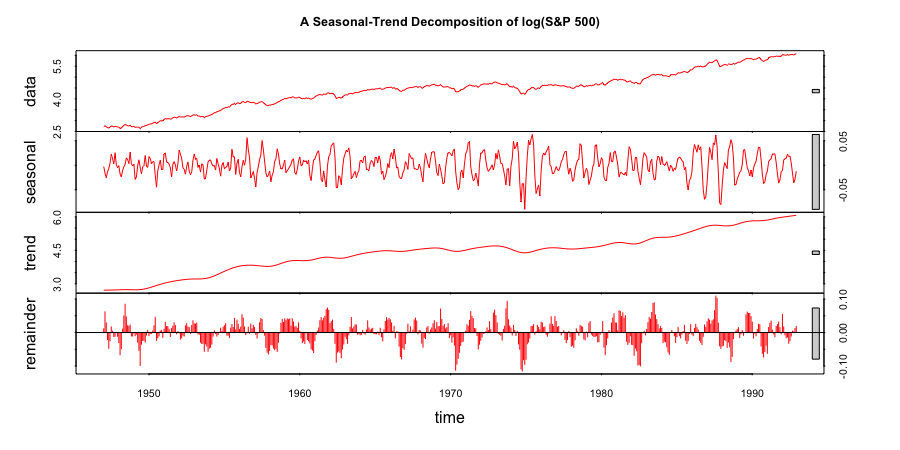
\includegraphics[scale=.5]{Images/STLSP500}
\caption{STL of Log SP500. a) The natural log of the SP500 b) The cyclical (or called seasonal) pattern c) The business trend of log SP500 d) Noise (remainder) data. The graph was created using the R program named as llt.R and it is attached in the Appendix A.}
\label{fig:STLSP500}
\end{figure}

A STL writes as $Y_t$, 

\begin{equation}
Y_t = f(S_t,T_t,E_t)
\end{equation} where $Y_t$ is time series data at time $t$, $S_t$ is seasonal component at time $t$, $T_t$ is trend component at time $t$ and $E_t$ is remainder (or error or irregular) component of data at time $t$ and $f$ is some function. For an additive decomposition $Y_t$ split up by
\begin{equation}
Y_t = S_t+T_t+E_t
\end{equation}

The user controls the variations on the trend and seasonal components.

In figure \ref{fig:STLSP500}, trend, seasonal and noise or error remainder data of the log of SP500 are extracted using the seasonal trend decomposition procedure. The seasonal window, in this case the value used is 5, is used to control the variation of the seasonal component. 


\begin{figure}[!ht]
\centering
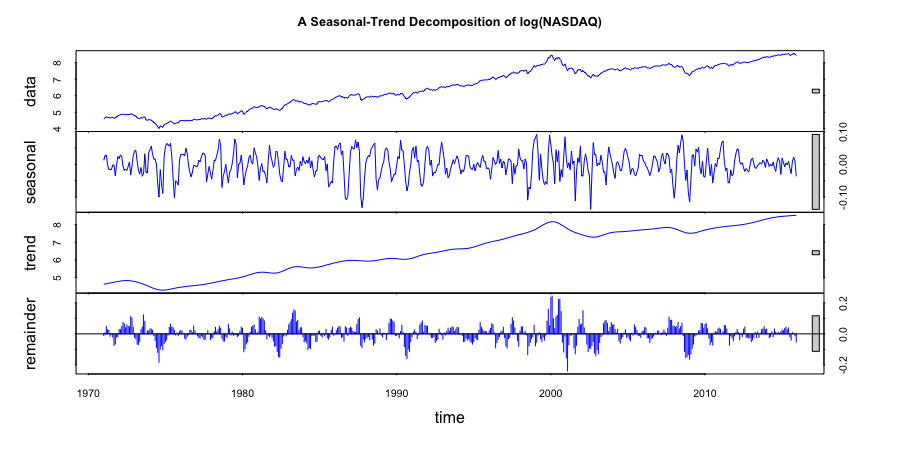
\includegraphics[scale=.5]{Images/STLNASDAQ}
\caption{STL of NASDAQ. a) The natural log of the NASDAQ b) The cyclical (or called seasonal) pattern c) The business trend of log NASDAQ d) Noise (remainder) data. The graph was created using the R program named as llt.R and it is attached in the Appendix A}
\label{fig:STLNASDAQ}
\end{figure}

In the figure \ref{fig:STLNASDAQ}, trend, seasonal and noise or error remainder data of the log of NASDAQ are extracted using the seasonal trend decomposition procedure. The seasonal window $(value = 5)$ is used to control the variation of the seasonal component. 

\subsection{Log-Linear Method}

When natural log values are used for the dependent variable and the independent variable is kept in its original scale, those models are called log linear models. 

The following model is of the value in a savings fund that depends on initial investment, growth rate and time duration in which the funds are invested. 

\begin{equation}
Y_t = Y_0{(1+r)}^t
\end{equation}
where $Y_t$ represents the value of the fund at the time $t$, $Y_0$ is the initial investment in the saving fund, and r is the growth rate.

\begin{figure}[!ht]
\centering
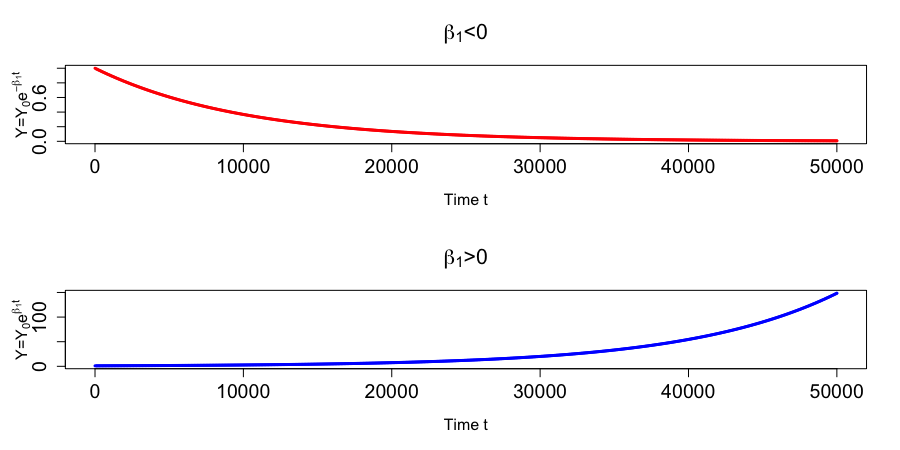
\includegraphics[scale=.5]{Images/LogLinear}
\caption{Log Linear Model when $\beta_1 < 0$ and when $\beta_1 > 0$. The graph was generated using loglinear.R, and it is attached in the Appendices A}
\label{fig:LogLinear}
\end{figure}
Taking log on both side, we obtain the following. 
\begin{equation}
log Y_t = log Y_0 + t log (1+r)
\end{equation}
Here $log Y_0$ is a constant and is taken to be $\beta_0$. Then $log (1+r)$ is taken to be $\beta_1$ and $log Y_t$ is given below:

\begin{equation}
log Y_t = {\beta}_0 + {\beta}_1 t
\end{equation}

\begin{figure}[!ht]
\centering
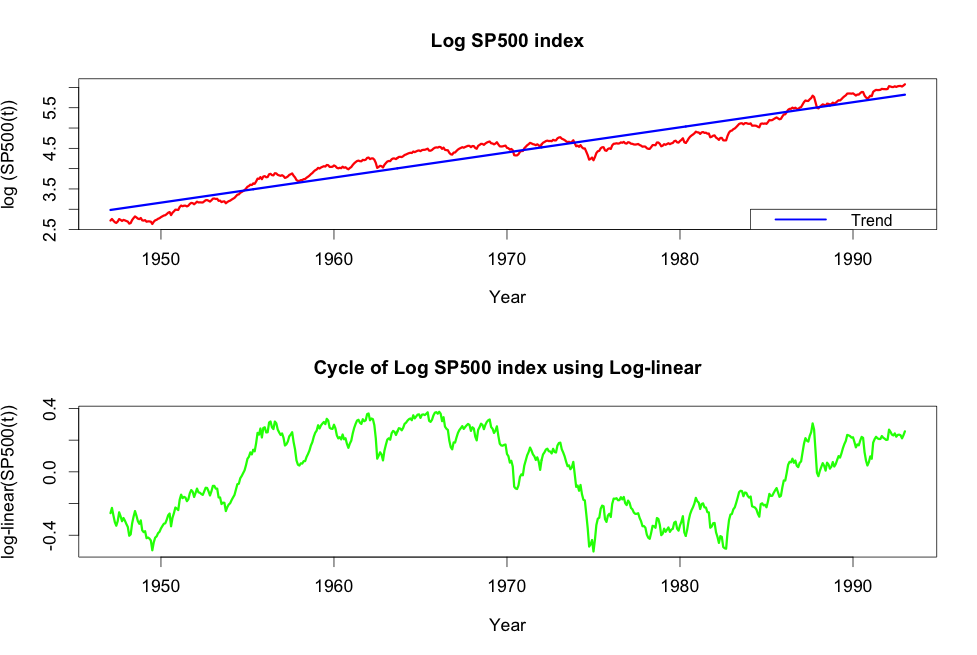
\includegraphics[scale=.5]{Images/lltcsp500}
\caption{Log linear of trend and cycle for log SP500 a) Log SP500 and trend. The trend is calculated based on estimation of slope and y-intersect  b)It is cycle of log-linear of SP500 and it is the variance of original log(sp500) and estimated trend. AutoCorrelation.R is the R program used to created the graph and it is attached in the Appendix A}
\label{fig:ACSP500}
\end{figure}

\begin{figure}[!ht]
\centering
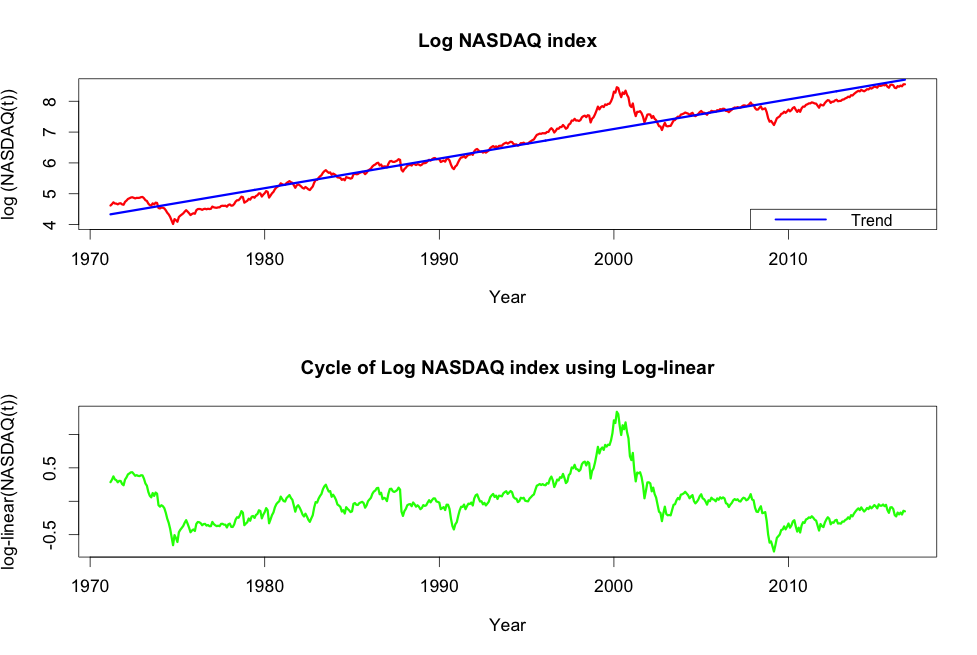
\includegraphics[scale=.5]{Images/lltcnasdaq}
\caption{Log linear of trend and cycle for log NASDAQ a) Log NASDAQ and trend. The trend is calculated based on estimation of slope and y-intersect  b)It is cycle of log-linear of SP500 and it is the difference between the original log(NASDAQ) and estimated trend. AutoCorrelation.R is the R program used to created the graph and it is attached in the Appendix A}
\label{fig:ACNASDAQ}
\end{figure}


After estimation of the log-linear model, the coefficients can be used to determine the impact of the independent variable $(t)$ on the dependent variable $(Y)$. The coefficient ${\beta}_1$ in a log-linear model represents the estimated percent change in the dependent variable for a unit change in independent variable. The coefficient ${\beta}_1$ provides the instantaneous rate of growth. The regression coefficients in the log-linear model do not represent the slope. 

When ${\beta}_1 > 0$, the log-linear function illustrates a positive impact from the independent variable and when, ${\beta}_1 < 0$, the log-linear function depicts a negative impact from the independent variable. 

\subsection{Auto correlation Functions}
An autoregressive model is when a value from a time series is regressed on previous value from that same time series. For exampe, $y_t$ on $y_{t-1}$:

\begin{equation}
y_t = \beta_{0} +\beta_{1}y_{t-1} +\epsilon_t
\end{equation}

In this regression model, the response variable in the previous time period has become the predictor and the errors have the same assumptions about errors in a simple linear regression model. The order of an autoregression is the number of immediate preceding values in the series that are used to predict the value at the present time. So, the preceding model is a first-order autoregression, written as $AR(1)$.

\begin{figure}[!ht]
\centering
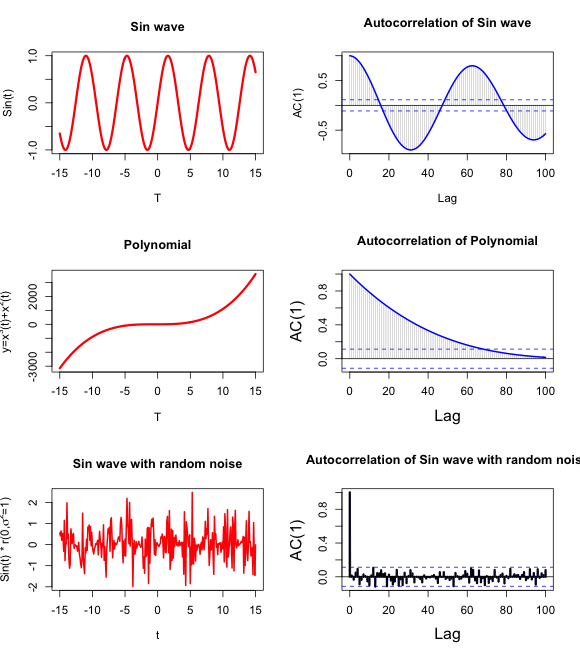
\includegraphics[scale=.65]{Images/ACExample}
\caption{Auto correlation for a) Sin wave b) Polynomial equation c) Sin wave with random noise. AutoCorrelation.R is the R program used to created the graph and it is attached in the Appendix A}
\label{fig:ACExample}
\end{figure}
\begin{figure}[!ht]
\centering
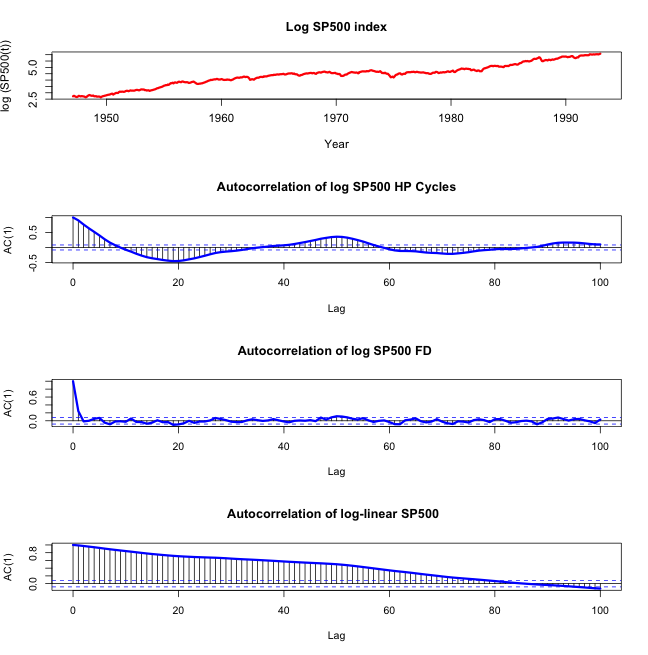
\includegraphics[scale=.65]{Images/ACSP500}
\caption{Auto correlation for log SP500 a) Log SP500 b)AutoCorrelation of HP cycle  c) Autocorrelation of First Differencing d) Autocorrelation of log-linear cycles of SP500. AutoCorrelation.R is the R program used to created the graph and it is attached in the Appendix A}
\label{fig:ACSP500}
\end{figure}
Let us say, if we want to predict the temperature $y$ this year $(y_t)$ using measurement of global temperature in the previous two years $(y_{t-1},y_{t-2})$. Then the autoregressive model for doing so would be:
\begin{equation}
y_t = \beta_{0} +\beta_{1}y_{t-1} +\beta_{2}y_{t-2}+\epsilon_t
\end{equation}

The above model is a second-order autoregression, written as $AR(2)$, since the value at time $t$ is predicted from the values at times $t-1$ and $t-2$. More generally, $k^{th}$ order autoregression, written as $AR(k)$, is a multiple linear regression in which the value of the series at any time $t$ is a linear function of the values at times $t-1,t-2,...,t-k$.

\begin{figure}[!ht]
\centering
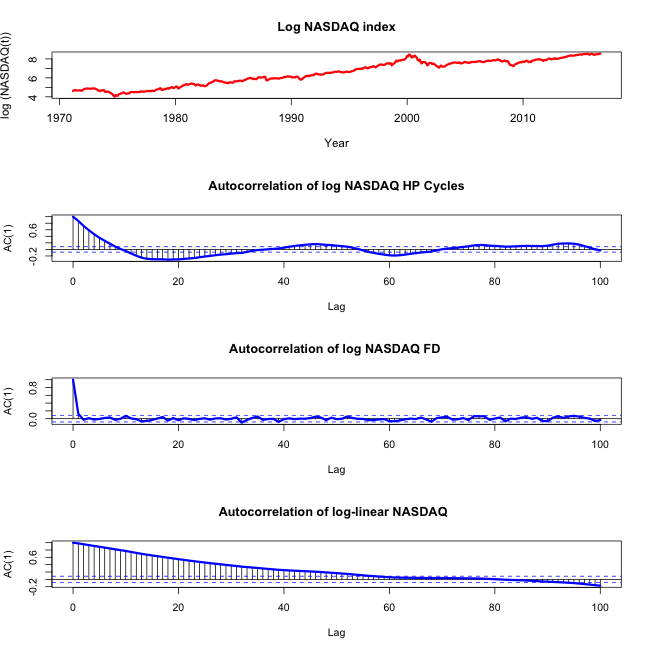
\includegraphics[scale=.65]{Images/ACNASDAQ}
\caption{Auto correlation for log NASDAQ a) Log NASDAQ b)AutoCorrelation of HP cycle  c) Autocorrelation of First Differencing d) Autocorrelation of log-linear cycles of NASDAQ. AutoCorrelation.R is the R program used to created the graph and it is attached in the Appendix A}
\label{fig:ACNASDAQ}
\end{figure}
The cofficient of correlation between two values in a time series is called the \textbf{autocorrection function} $(ACF)$. Let $y_t$ be a sample, $t = 1,2,..,n$ from an ARMA process of possibly unknown order, then the $j^{th}$ order auto correlation $\rho(j)$ can be esimated by using the formula
\begin{equation}
\rho(j) = \frac{Cov(y_t,y_{t-j})}{Var(y_t)}
\end{equation}
where
\begin{equation}
Cov(y_t,y_{t-j}) = \frac{1}{n-1} \sum_{t=j+1}^{n}(y_t-y_\mu)(y_{t-j}-y_\mu)
\end{equation}
\begin{equation}
Var(y_t)= \frac{1}{n-1} \sum_{t=1}^{n}(y_t-y_\mu)^2
\end{equation}
$y_\mu$ is the mean of the $y_t$.
\subsection{Hodrick and Prescott (HP) filter}
Hodrick and Prescott proposed the HP filter to decompose a macroeconomic time series into a non-stationary trend component and a stationary cyclical residual component. The filter has become popular in applied macro economics in the last 15 years.  Given an observed series $y_i$, let $y_i = x_i + c_i$, with $y^T = (y_1,y_2..., y_N), x^T = (x_1,x_2,....x_N)$ and $c^T = (c_1,c_2...., c_N)$ where $x_t$ denotes the unobserved trend component at time $t$ and $c_t$ the unobserved cyclical residual at time $t$. The HP trend $\hat{x}$ can be obtained as the solution to the following convex minimization problems:



\begin{equation}
\min_{[x_t]_{t=1}^{N}}  \begin{bmatrix} \sum_{t=1}^{N} (y_t - x_t)^2 +\lambda \sum_{t=2}^{N-1} ( ( x_{t+1} - x_t) - (x_t - x_{t-1}))^2  \end{bmatrix}
\end{equation}

Here, $\lambda$ is usually known as the smoothing parameter. As $\lambda$ becomes larger, the HP estimated trend curve becomes smoother. The term being squared in the second sum of the equation, $( x_{t+1} - x_t) - (x_t - x_{t-1})$, or $\bigtriangleup^{2}x_i$, is an approximation to the second derivate of $x$ at time $t$. There are two opposing forces in the HP minimization problem. One force is attempting to minimize the sum of squared cyclical residuals and the other force is attempting to minimize the sum of squared $\bigtriangleup^{2}x_i$. The smoothing parameter, $\lambda$, gives relative weight to these two opposing forces. 

\begin{table}[h!]
\centering
\begin{tabular}{||c c c c c c ||} 
 \hline
 Detrending & Mean & SD & Variance & $T_{0}$ (month) & $P_{dc}$ (year) \\ [0.5ex] 
 \hline\hline
 FD & 0.011 & 0.1123 & 0.0126 & 1.94 & 00.7 \\
 HP & 0.008 & 0.2686 & 0.0722 & 8.93 & 02.9 \\
 LLD & 0.426 & 0.3265 & 0.1066 & 85.6 & 28.5  \\
 \hline
\end{tabular}
\caption{Detrend Statistics on S\&P 500. The value for the above table was created by using the Matlab program DetrendStatistics.m attached in the appendix.  }
\label{table:sp500trendstat}
\end{table}


\begin{table}[h!]
\centering
\begin{tabular}{||c c c c c c ||} 
 \hline
 Detrending & Mean & SD & Variance & $T_{0}$ (month) & $P_{dc}$ (year) \\ [0.5ex] 
 \hline\hline
 FD & 0.008 & 0.1072 & 0.0115 & 1.81 & 00.6 \\
 HP & 0.022 & 0.2256 & 0.0509 & 9.22 & 03.0 \\
 LLD & 0.258 & 0.3159 & 0.0992 & 80.5 & 26.8  \\
 \hline
\end{tabular}
\caption{Detrend Statistics on NASDAQ. The value for the above table was created by using the Matlab program DetrendStatistics.m attached in the appendix.  }
\label{table:sp500trendstat}
\end{table}

The $\lambda$ parameter determines the smoothness of the trend component. The larger the value of $\lambda$, the higher the penalty in the  second term.  An empirical study indicates that a $5\%$ cyclical component is moderately large, as is a $1/8$th of $1\%$ change in the growth rate in a quarter. In the paper \cite{lambdaforhp}, $\lambda$ should be adjusted by multiplying it with the fourth power of the observation frequency ratios. This yields an HP parameter value of 6.25 for annual data given a value of 1600 for quarterly data. 

\subsubsection{First-order conditions of the HP minimization problem}

The following HP first order conditions are derived by setting the gradient vector of the above minimization equation equal to zero. The first-order conditions are:
\begin{flushleft}
\begin{align}
c_1&=\lambda(x_1-2x_2+x_3)  \nonumber \\
c_2&=\lambda(-2x_1+5x_2-4x_3+x_4) \nonumber \\
c_t&=\lambda(x_{t-2}-4x_{t-1}+6x_t-4x_{t+1}+x_{t+2}), t=3,4,5,....,N-2 \nonumber \\
c_{N-1}&=\lambda(x_{N-3}-4x_{N-2}+5x_{N-1}-2x_N) \nonumber \\
c_{N}&=\lambda(x_{N-2}-2x_{N-1}+x_N) \nonumber
\end{align}
\end{flushleft}
or more compactly, 
\begin{center}
\boldmath{$c=\lambda Fx$}
\end{center}
\unboldmath
where F = 
\begin{flushright}
$\begin{bmatrix}
1 & -2 & 1 & 0 & \cdots & \cdots & \cdots &\cdots & & 0 \\
-2 & 5 & -4 & 1 & 0 & \cdots & \cdots & & & 0 \\
1 & -4 & 6 & -4 & 1 & 0 & \cdots &  & & 0 \\
0 & 1 & -4 & 6 & -4 & 1 & 0 & \cdots & &  0 \\
0 & 0 & 1 & -4 & 6 & -4 & 1 & 0  &\cdots  & 0 \\
\vdots & & & & & & & & & \vdots \\
\vdots & & & & & & & & & \vdots \\
\vdots & & & & & & & & & \vdots \\
0 & \cdots & \cdots & 0 & 1 & -4 & 6 & -4 & 1 & 0 \\
0 & \cdots & & \cdots &   0 & 1 & -4 & 6 & -4 & 1 \\
0 & \cdots & \cdots &  &  & 0 & 1 & -4 & 5 & -2 \\
0 & \cdots & \cdots & \cdots &  &  & 0& 1 & -2 & 1 
\end{bmatrix}$
\end{flushright}

which implies that 

\begin{center}
\boldmath{$y=(\lambda F+I)x$}
\unboldmath
\end{center}
Thus, the HP trend is given by:
\begin{center}
\boldmath{$\hat{x}=(\lambda F+I)^{-1}y$}
\unboldmath
\end{center}
and
\begin{center}
\boldmath{$\hat{c}=y-\hat{x}$}
\unboldmath
\end{center}

\begin{figure}[!ht]
\centering
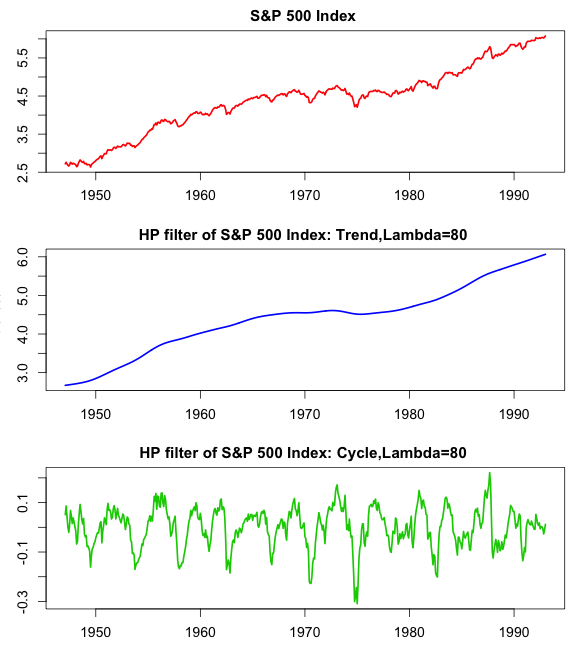
\includegraphics[scale=.65]{Images/SP500HP80}
\caption{The trend and cycle separation from SP500 using HP filter with $\lambda$ = 80. a) Natural Log of SP500 index b) Trend extracted from Log of SP500 index using HP filter c) Cyclical pattern extracted from SP500 index using HP filter}
\label{fig:SP500HP80}
\end{figure}

In the figure \ref{fig:SP500HP80}, the $\lambda$ value is 80 and the trend and cyclical information is separated from the natural log SP500 index and the trend data is useful for the long term investors like pension fund manager. The long term fund managers require the projection of the performance of an index to strategize the investment to meet the client's retirement objective. 

\begin{figure}[!ht]
\centering
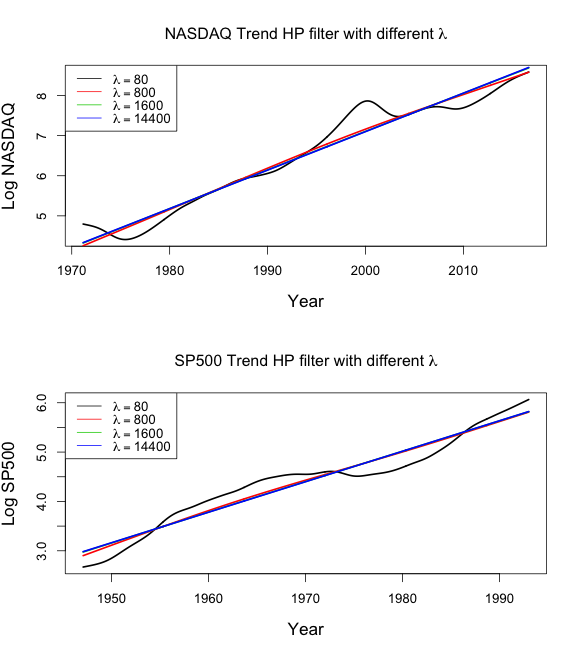
\includegraphics[scale=.65]{Images/Lambda}
\caption{HP filter with different value for $\lambda$ a) NASDAQ b) S\&P 500}
\label{fig:Lambda}
\end{figure}
In the figure \ref{fig:Lambda}, the SP500 trend analysis was performed using different $\lambda$ values. The trend looks very similar when the $\lambda$ is above 800 value and there is no significance when the $\lambda$ values are at 1600, 14400. The above figure \ref{fig:Lambda}, indicates that when $\lambda$ is above 800 or above the trend in the HP filter is very close to least square linear regression line. 

\begin{figure}[!ht]
\centering
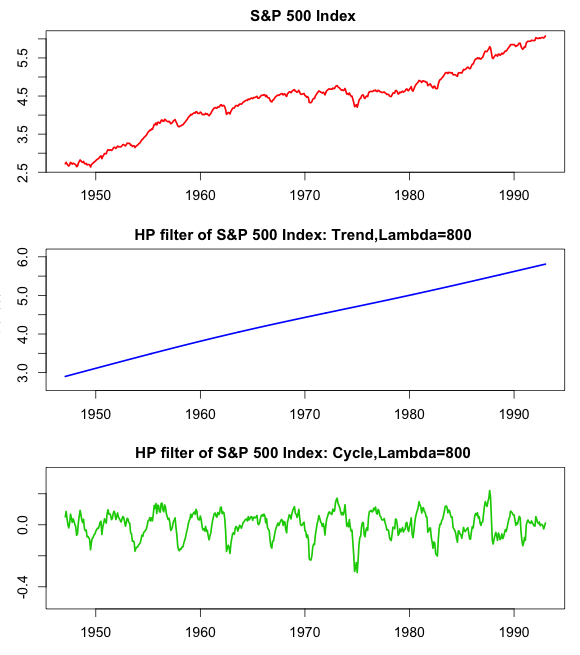
\includegraphics[scale=.65]{Images/SP500HP800}
\caption{The trend and cycle separation from SP500 using HP filter with $\lambda$ = 800. a) Natural Log of SP500 index b) Trend extracted from Log of SP500 index using HP filter c) Cyclical pattern extracted from SP500 index using HP filter }
\label{fig:SP500HP800}
\end{figure}
In the figure \ref{fig:SP500HP800}, the $\lambda$ value is 800  and a similar analysis was performed.


\begin{figure}[!ht]
\centering
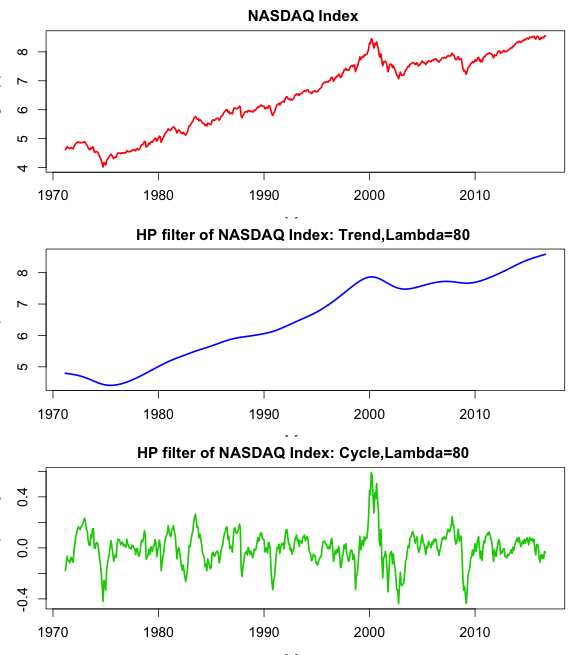
\includegraphics[scale=.65]{Images/NASDAQHP80}
\centering
\caption{The trend and cycle separation from NASDAQ using HP filter with $\lambda$ = 80. a) Natural Log of NASDAQ index b) Trend extracted from Log of NASDAQ index using HP filter c) Cyclical pattern extracted from NASDAQ index using HP filter }
\label{fig:NASDAQHP80}
\end{figure}
In the figure \ref{fig:NASDAQHP80}, the $\lambda$ value is 80 and the trend and cyclical information is separated from the natural log NASDAQ index.


In the figure \ref{fig:Lambda}, the NASDAQ trend analysis was performed using different $\lambda$ values. The trend looks very similar when the $\lambda$ is above 800 value and there is no signficance when the $\lambda$ values are at 1600, 14400.
\begin{figure}[!ht]
\centering
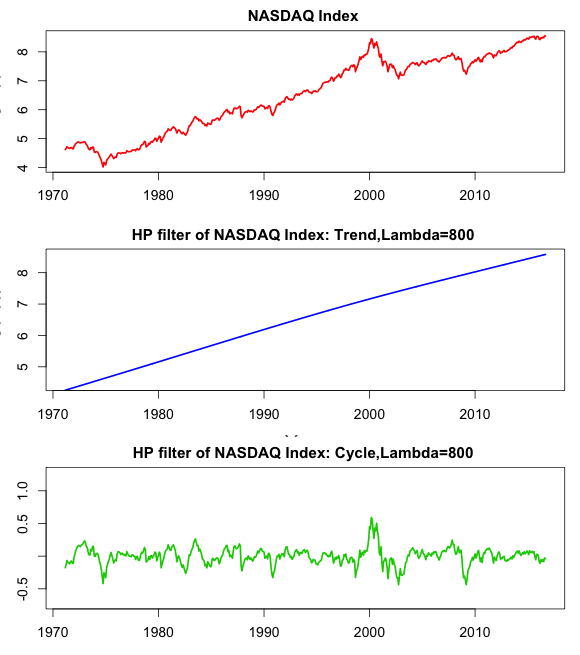
\includegraphics[scale=.65]{Images/NASDAQHP800}
\caption{The trend and cycle separation from NASDAQ using HP filter with $\lambda$ = 800. a) Natural Log of NASDAQ index b) Trend extracted from Log of NASDAQ index using HP filter c) Cyclical pattern extracted from NASDAQ index using HP filter }
\label{fig:NASDAQHP800}
\end{figure}

The HP filters is one of the most heavily used econometric methods for measuring business cycles and potential output in empirical research. It is also a smoothing method that belongs to a very general class of nonparametric graduation procedures that depend on a tuning parameter governing the properties of the smoother. The long run potential output of an economy can be substantially influenced by great recessions and depressions, which may sufficiently divert resources to impact long run trend components of output. The HP filter has the advantage that, depending on the smoothing parameter $(\lambda)$ choice, it can encompass long run behavior that encompasses a vast range of possibilities -from a deterministic linear trend, to a smooth Gaussian process, through to stochastic trends and combination of stochastic trends and deterministic trends that even include trend breaks. 

